\documentclass[journal,12pt,twocolumn]{IEEEtran}
\usepackage[utf8]{inputenc}
\usepackage{amsmath}   
\usepackage{graphicx}

\begin{document}

\newcommand{\myvec}[1]{\ensuremath{\begin{pmatrix}#1\end{pmatrix}}}

\let\vec\mathbf


\title{Assignment 1}
\author{\textbf{Himanshu Kumar Gupta(AI21BTECH11012)}}
\maketitle
\date {March 2022}


\textbf{\textit{Problem 3b, ICSE 10 2019:}}


 M and N are two points on the X axis and Y axis respectively. 
P (3, 2) divides the line segment MN in the ratio 2 : 3.

Find:
\begin{enumerate}
    \item The coordinates of M and N
    \item Slope of the line MN
\end{enumerate}

\textbf{\textit{Solution:}}

	The various parameters involved in this question are listed in Table \eqref{table:1}:
	\begin{table}[ht!]
		\begin{tabular}{|l|c|c|}

\hline
\textbf{Parameter} & \textbf{Symbol/Formula} & \textbf{Value} \\
\hline
standard vector 1 & $\vec{e_1}$ & $\myvec{1\\0}$ \\
\hline
standard vector 2 & $\vec{e_2}$ & $\myvec{0\\1}$ \\
\hline
position vector of point P & $\vec{P}$ & $\myvec{3\\2}$ \\
\hline
position vector of point M & $\vec{M}$ & $\myvec{p\\0}$\\
\hline
position vector of point N & $\vec{N}$ & $\myvec{0\\q}$\\
\hline

\end{tabular}

		\vspace{5pt}
		\caption{}
		\label{table:1}	
	\end{table}

  from section formula in vector form, we know that
  
  \begin{equation}
  \label{eq:1}
\vec{P}=\frac{1\times \vec{M} +k\times \vec{N}}{1+k}     
  \end{equation}
 
  where k:1 is ratio in which point P divides the line joining M and N
  
Since P(3,2) divides M and N in ratio 2:3

So,$ k=\frac{2}{3}$

Now,by applying section formula given in equation \eqref{eq:1} to P on line MN, we get

\begin{align}
    &\vec{P}=\frac{1\times \vec{M}+\frac{2}{3}\times \vec{N}}{1+\frac{2}{3}}\\
    &\implies  3\times\vec{e_1}+2\times\vec{e_2} =\frac{1\times (p\times \vec{e_1})+\frac{2}{3}\times (q\times\vec{e_2})}{\frac{5}{3}}\\
   &\implies 3\times\vec{e_1}+2\times\vec{e_2}=\frac{3\times (p\times\vec{e_1})+2\times (q\times\vec{e_2})}{5}\\
  &\implies 15\times\vec{e_1}+10\times\vec{e_2}=3p\times\vec{e_1}+2q\times\vec{e_2}\\
\label{eq:6}
 &\implies (15-3p)\times \vec{e_1}+(10-2q)\times\vec{e_2}=0
\end{align}
Now,coefficient of $\vec{e_1}$ and $\vec{e_2}$ in equation\eqref{eq:6} should be independently equal to 0,
So,
\begin{equation*}
3p-15=0\quad 2q-10=0
\end{equation*}
\begin{equation*}
 \implies3p=15\quad  \implies2q=10
\end{equation*}
\begin{equation}
 \implies p=5\quad \implies q=5      
\end{equation}
So,the vectors $\vec{M}=5\times\vec{e_1}+0\times\vec{e_2}=\myvec{5\\0}$ and $ \vec{N}=0\times\vec{e_1}+5\times\vec{e_2}=\myvec{0\\5}$ 
 
therefore the points M and N would be \textbf{(5,0)} and \textbf{(0,5)} respectively.
\begin{figure}[htb!]
\centering
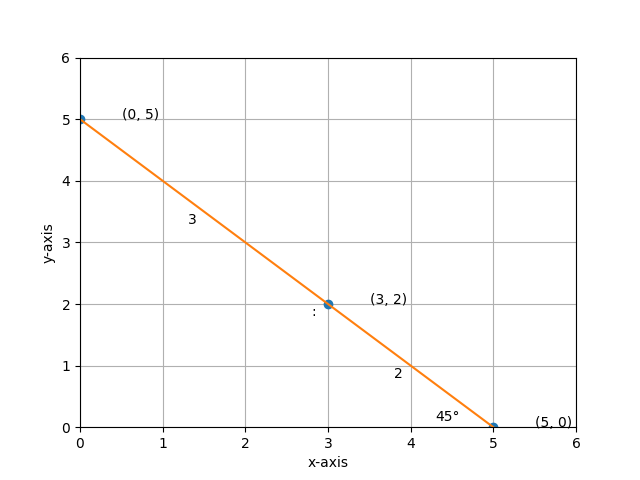
\includegraphics{figures/Figure_1(1).png}
\caption{graph representing M,N and P}
\end{figure}

Now,the vector         
\begin{align}
\vec{MN}&=\vec{N}-\vec{M}\\
&=(0\times\vec{e_1}+5\times\vec{e_2})-(5\times\vec{e_1}+0\times\vec{e_2})\\
&=-5\times\vec{e_1}+5\times\vec{e_2}
\end{align}

Now,we know that the slope of any vector is
\begin{align}
    &= \dfrac{\text{coefficient of $\vec{e_2}$}}{\text{coefficient of $\vec{e_1}$ }}
\end{align}
So,slope of $\vec{MN}$,
 \begin{align}
  slope &=\frac{5}{-5}\\
  &=\textbf{-1}             
\end{align}


\end{document}
